\documentclass[final,narroweqnarray,inline]{ieee}
% In order to use the figure-defining commands in ieeefig.sty...
\usepackage{ieeefig}
% To use utf8 encoding
%\usepackage[T1]{fontenc}
\usepackage[utf8]{inputenc}
%\usepackage[spanish]{babel}
\begin{document}

%----------------------------------------------------------------------
% Title Information, Abstract and Keywords
%----------------------------------------------------------------------
\title[Trabajo Práctico N$^o$ 1: Wiretapping]{%
Trabajo Práctico N$^o$ 1: Wiretapping}

% format author this way for journal articles.
\author[SHORT NAMES]{%
	Leandro Ezequiel Barrios,
	\and
	Gonzalo Benegas,
	\and
	Martin Caravario, 
	\and
	Pedro Rodriguez 
}

% make the title
\maketitle

% do the abstract
\begin{abstract}

En el presente Trabajo Práctico utilizaremos algunas de las técnicas
provistas por la teoría de la información para estudiar y analizar
algunas redes de información. El objetivo será distinguir diversos
aspectos de la red de manera analítica. Para cumplir con nuestro
objetivo, haremos uso de dos herramientas modernas de manipulación y
análisis de paquetes: Wireshark y Scapy.

\end{abstract}

% start the main text ...

%----------------------------------------------------------------------
% SECTION I: Introduction
%----------------------------------------------------------------------
\section{ Introducción }

Construimos una herramienta que hace uso de la función
\texttt{``sniff''}, provista por la librería \textbf{Scapy} de
Python. Esta nos permitió activar el \texttt{modo promiscuo}, o
\texttt{monitor} en el caso de las placas wireless. Esto nos permitió
escuchar la red durante cierto tiempo, obteniendo todos los paquetes
que llegaban a nuestra placa de red. A partir de estos datos que
guardamos en un archivo \texttt{pcap}, se definieron dos fuentes de
información, con las cuales fuimos capaces de encontrar nodos y
protocolos distinguidos en la red. Para su visualización, elegimos la
realización de gráficos de torta e histogramas, ya que los
consideramos los más apropiados.

Para cada una de las mediciones consideramos las siguientes fuentes: 
\begin{itemize}

  \item $S = \{s_{1} \dots s_{n}\}$, provista por la cátedra, donde
  $s_{i}$ es el valor del campo \emph{type} de cada paquete de capa
  2.

  \item $S_{1} = \{s_{1} \dots s_{n}\} $, determinada por nosotros,
  donde $s_i$ es el valor del campo destino (MAC) cada paquete de
  capa 2 de tipo ARP.

\end{itemize}

\medskip

Para entender qué es lo que se obtendrá al efectuar estas mediciones,
hay que aclarar que \texttt{ARP} es un protocolo de la capa de enlace
de datos, responsable de encontrar la dirección de capa 2
(\texttt{Ethernet MAC}) que corresponde a una determinada dirección IP
(dirección de capa 3 de enlace).

Es decir, cada vez que un host quiere comunicarse con otro y su
dirección \texttt{MAC} no se encuentra dentro de su tabla
\texttt{ARP}, debe enviar un paquete who-has broadcast para determinar
la dirección \texttt{MAC} del host destino. De este modo, todos los
hosts del dominio de colisión de la máquina en la que se efectúa la
medición reciben dicho paquete, siendo respondido el mismo únicamente
por el host requerido, mediante un paquete \emph{reply}.

Para distinguir \emph{nodos} (símbolos) en este contexto, tomamos a
aquellos cuya probabilidad de aparición era alta, de forma tal que la
información provista por el mismo fuera menor a la entropía de la
fuente a la cuál el símbolo pertenecía.

\newpage
%----------------------------------------------------------------------
% SECTION II: Desarrollo - Fuente S
%----------------------------------------------------------------------
\section{Desarrollo - Fuente S}
  %--------------------------------------------------------------------
  % SUBSECTION II-A: CASA
  %--------------------------------------------------------------------
  \subsection{Casa}

  %--------------------------------------------------------------------
  % SUBSECTION II-B: TECHINT
  %--------------------------------------------------------------------
  \subsection{Techint}
  Esta medición fue realizada en la empresa Techint, en el horario de las
  11:00 am, por un lapso de 30 minutos. Se utilizó la herramienta
  desarrollada en el ejercicio anterior. 

  
  Como se observa en la figura TORTA, el protocolo que mas aparece en
  este escenario es \texttt{IPv4}, haciendo que su probabilidad sea la
  mayor. Esto se ve reflejado en la figura HISTOGRAMA, en la cual se puede
  ver como afecta la frecuencia de aparición del protocolo a la información
  que este provee.

  En este caso el nodo distinguido es el protocolo \texttt{IPv4}, pues la
  información que provee es menor a la entropía de la fuente. 
  %--------------------------------------------------------------------
  % SUBSECTION II-C: HYUNDAI
  %--------------------------------------------------------------------
  \subsection{Hyundai}

  %--------------------------------------------------------------------
  % SUBSECTION II-D: LABORATORIOS DC
  %--------------------------------------------------------------------
  \subsection{Laboratorios DC}

  %--------------------------------------------------------------------
  % SUBSECTION II-E: Gráficos
  %--------------------------------------------------------------------
  \subsection{Gráficos}
  \subsubsection*{Gráficos Torta}
  %casa
    \begin{figure}[ht]\begin{center}
      %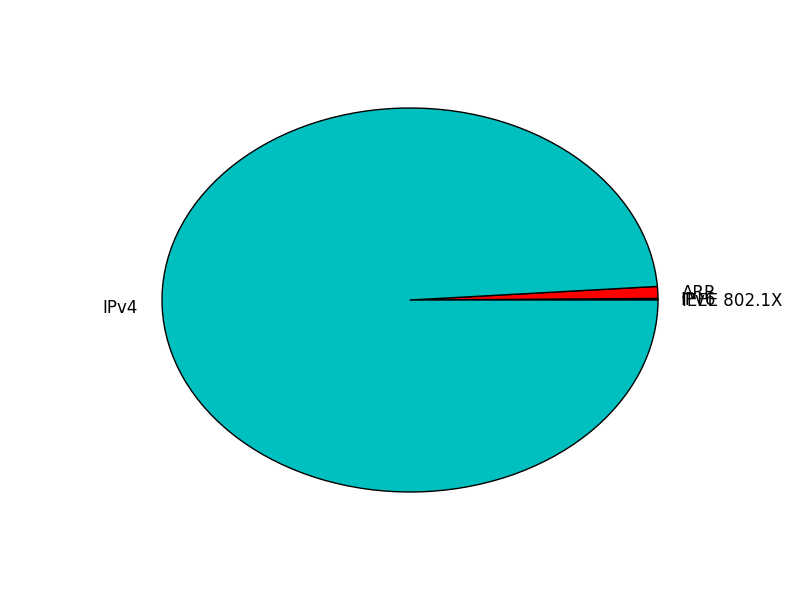
\includegraphics[width=0.5\textwidth]{../output/marto-casa-3hs-s-pie.png}
      \caption{S: Casa - Torta}
      \label{marto-casa-3hs-s-pie}
    \end{center}\end{figure}
  % techint
  \includegraphics[width=0.5\textwidth]{../output/dummy-s-pie.png}
  \includegraphics[width=0.5\textwidth]{../output/dummy-s-pie.png}
    \begin{figure}[ht]\begin{center}

    \end{center}\end{figure}
  % hyundai
  % laboratorios dc

  \subsubsection*{Gráficos Histograma}
  % casa
    \begin{figure}[ht]\begin{center}
      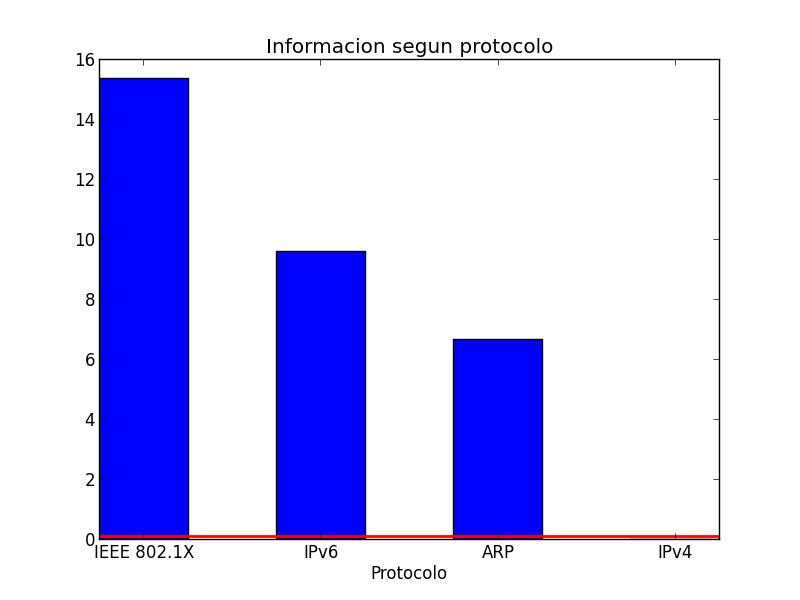
\includegraphics[width=0.5\textwidth]{../output/marto-casa-3hs-s-histogram.png}
      \caption{S: Casa - Histograma}
      \label{marto-casa-3hs-s-histogram}
    \end{center}\end{figure}
  % techint
    \begin{figure}[ht]\begin{center}
      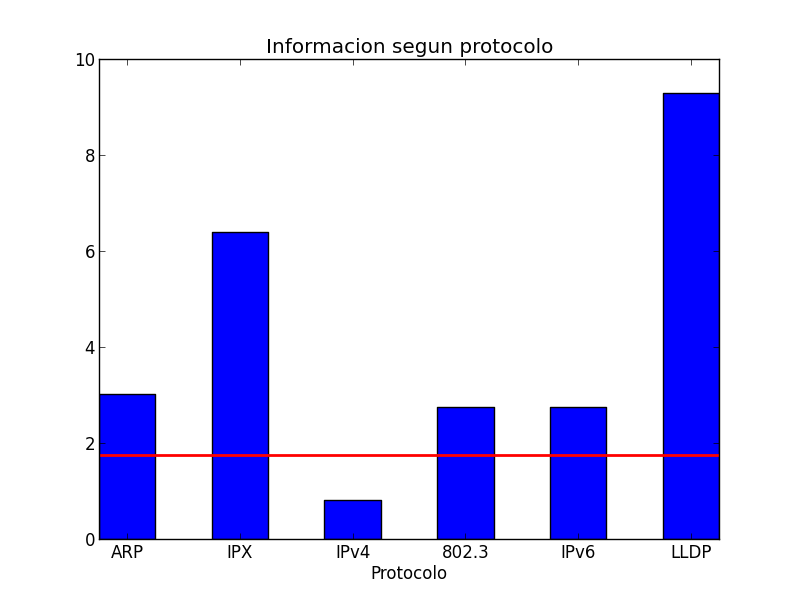
\includegraphics[width=0.5\textwidth]{../output/techint-s-histogram.png}
      \caption{S: Techint - Histograma}
      \label{techint-s-histogram}
    \end{center}\end{figure}
  % hyundai
    \begin{figure}[ht]\begin{center}
      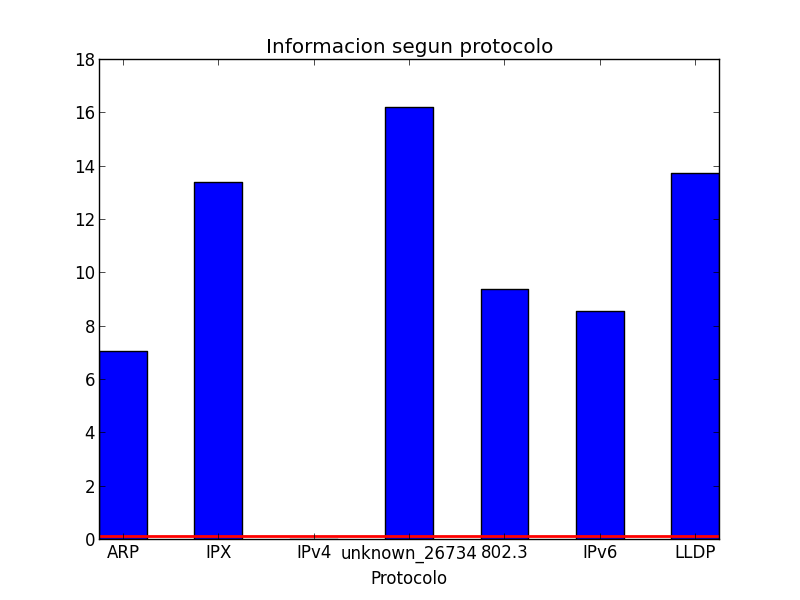
\includegraphics[width=0.5\textwidth]{../output/hyundai-s-histogram.png}
      \caption{S: Hyundai - Histograma}
      \label{hyundai-s-histogram}
    \end{center}\end{figure}
  % laboratorios dc
    \begin{figure}[ht]\begin{center}
      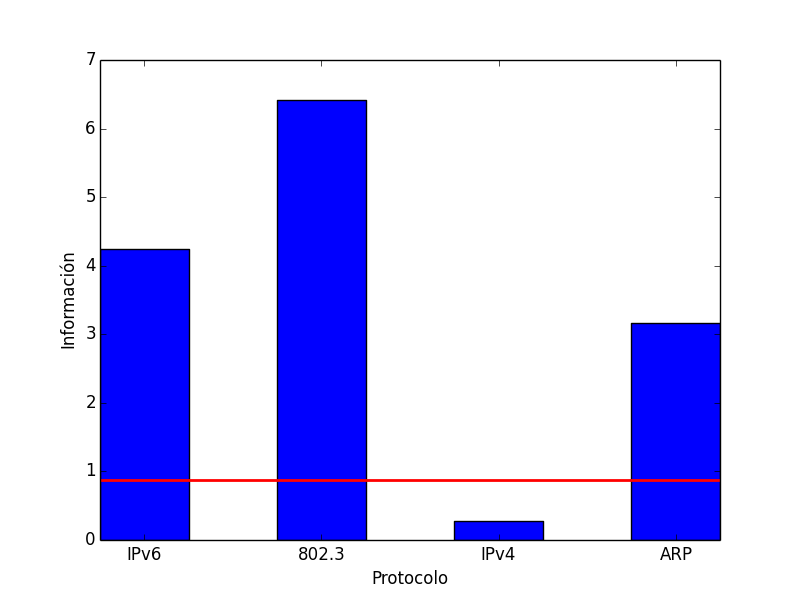
\includegraphics[width=0.5\textwidth]{../output/labos-dc-30m-s-histogram.png}
      \caption{S: Laboratorios DC - Histograma}
      \label{labos-dc-30m-s-histogram}
    \end{center}\end{figure}


  %--------------------------------------------------------------------
  % SUBSECTION II-F: Conclusión
  %--------------------------------------------------------------------
  \subsection{Conclusión}

\newpage
%----------------------------------------------------------------------
% SECTION III: Desarrollo - Fuente S
%----------------------------------------------------------------------
\section{Desarrollo - Fuente $S_1$}
  %--------------------------------------------------------------------
  % SUBSECTION II-A: CASA
  %--------------------------------------------------------------------
  \subsection{Casa}

  %--------------------------------------------------------------------
  % SUBSECTION II-B: TECHINT
  %--------------------------------------------------------------------
  \subsection{Techint}

  %--------------------------------------------------------------------
  % SUBSECTION II-C: HYUNDAI
  %--------------------------------------------------------------------
  \subsection{Hyundai}

  %--------------------------------------------------------------------
  % SUBSECTION II-D: LABORATORIOS DC
  %--------------------------------------------------------------------
  \subsection{Laboratorios DC}

  %--------------------------------------------------------------------
  % SUBSECTION II-E: Gráficos
  %--------------------------------------------------------------------
  \subsection{Gráficos}
  \subsubsection*{Gráficos Torta}
  \subsubsection*{Gráficos Histograma}

  %--------------------------------------------------------------------
  % SUBSECTION II-F: Conclusión
  %--------------------------------------------------------------------
  \subsection{Conclusión}

\newpage
%----------------------------------------------------------------------
% SECTION IV: Conclusión
%----------------------------------------------------------------------
\section{Conclusión}

% do the biliography:
%\bibliographystyle{IEEEbib}
%\bibliography{my-bibliography-file}

% where ``my-bibliography-file.bib'' is the name of the file with all the 
% BibTeX entries.

% do the biographies...
%\begin{biography}{Gregory L. Plett}
%  A bio with no face...
%\end{biography}

% If you want a picture with your biography, then specify the name of
% the postscript file in square brackets. That is, uncomment the
% following three lines and change the name of "face.ps" to the name of 
% your file.
%\begin{biography}[face.ps]{Gregory L. Plett}
%  A bio with a face...
%\end{biography}

\end{document}